\documentclass[12pt]{article}
\NeedsTeXFormat{LaTeX2e}

%%%%%%%%%%%%%%%%%%%%%%%%%%%%%%%%%%%%%%%%%

% Template by Nicholas Bertollo
% You may change and reuse this as you see fit

%%%%%%%%%%%%%%%%%%%%%%%%%%%%%%%%%%%%%%%%%

% Replace this information!
\newcommand{\studyunit}{MATH1064}
\newcommand{\studyperiod}{Semester 2, 2025}

%%%%%%%%%%%%%%%%%%%%%%%%%%%%%%%%%%%%%%%%%

\usepackage[svgnames]{xcolor}
\usepackage[T1]{fontenc}
\usepackage[margin=2.7cm,a4paper]{geometry}
\renewcommand{\baselinestretch}{1.15}

\usepackage[osf]{mathpazo}
\usepackage{amsmath,amsthm,amsfonts,amssymb,mathtools}

\usepackage{hyperref,url}
\usepackage{xstring}

\usepackage{environ}
\usepackage{tasks}

\usepackage{etoolbox}
\usepackage{fourier-orns}
\usepackage{kvoptions}
\usepackage[]{units}
% \usepackage[normal]{subfigure}
\usepackage{subfig}
\usepackage{array}

% Algorithms package

% \usepackage[ruled]{algorithm2e} % You can use the algorithm2e if you'd like
\usepackage[noend]{algpseudocode} % You may get rid of noend if you like. 
\usepackage{algorithm}
\usepackage{algorithmicx}

% No indents
\usepackage[parfill]{parskip}

% Tikz diagrams
\usepackage{tikz}
\usetikzlibrary{shapes.geometric,patterns,patterns.meta,arrows,positioning,fit,calc}
\pgfdeclarelayer{background}
\pgfsetlayers{background,main}

% Graphics and images
\usepackage{graphicx}
\graphicspath{ {./images/} }

% Header
\usepackage{fancyhdr}
\addtolength{\headheight}{2.5pt}
\pagestyle{fancy}
\fancyhead{} 
\fancyhead[L]{\sc \studyunit}
\fancyhead[R]{\sc \studyperiod}
\fancyfoot{}
\fancyfoot[R]{\thepage}
\renewcommand{\headrulewidth}{0.75pt}

%%%%%%%%%%%%%%%%%%%%%%%%%%%%%%%%%%%%%%%%%%%%%%%%%%%%%%%%%%%%%%%%%%%%%%%%%%%%%%%%%%

% Some basic mathematics commands!

\DeclarePairedDelimiter\ceil{\lceil}{\rceil}
\DeclarePairedDelimiter\abs{\lvert}{\rvert}

\newcommand{\lt}{\ensuremath <}
\newcommand{\gt}{\ensuremath >}
\newcommand{\Z}{\mathbb{Z}}
\newcommand{\N}{\mathbb{N}}
\newcommand{\R}{\mathbb{R}}
\newcommand{\Q}{\mathbb{Q}}
\newcommand{\U}{\mathbb{U}}
\newcommand{\compline}[1]{\overline{#1}}
\newtheorem{theorem}{Theorem}
\theoremstyle{definition}
\newtheorem{definition}{Definition}
\DeclareMathOperator{\lcm}{lcm}

%%%%%%%%%%%%%%%%%%%%%%%%%%%%%%%%%%%%%%%%%%%%%%%%%%%%%%%%%%%%%%%%%%%%%%%%%%%%%%%%%%

% Macros
% \newcounter{weekcntr}
% \newcommand*{\week}{
%     \stepcounter{weekcntr}
%     \section{Week \theweekcntr}
% }
    
 
\begin{document}
    \begin{titlepage}
        \begin{center}
            \vspace*{1cm}

            \section*{MATH1064 Study Notes}

            \vspace{0.25cm}
            University of Sydney \\
            \studyperiod \\
            \studyunit

            \vfill
            
\includegraphics{thumbs_up_emoji.png}
            \vspace{1.5cm}

            Happy studying!
            
       \vspace{0.8cm}
            
        \end{center}
    \end{titlepage}

    \tableofcontents
    
    \newpage
    \section{Introduction to Discrete Maths and Set Theory}
    \subsection{Introduction to Discrete Maths}

        Discrete maths is the study of "discrete structures", this includes objects which are:
        \begin{itemize}
            \item Countable or listable
            \item Distinct and unconnected.
        \end{itemize}

        There are two objectives of {\studyunit}:
        \begin{enumerate}
            \item Develop mathematical reasoning skills. This involves using \textbf{logic and proofs}, and 
            \textbf{rigorously} (exhausting all possibilities) finding solutions to problems.
            \item Study \textbf{discrete structures} and their properties including:
            \begin{itemize}
                \item Sets and functions
                \item Prime numbers and modular arithmetic
                \item Graphs and networks
                \item Counting and probability.
            \end{itemize}
        \end{enumerate}
    
        \subsection{Introduction to Set Theory}
        \subsubsection{Definitions}
        \begin{definition}[Set]
            \label{def:set}
            A \textbf{set} $S$ is a collection of objects, called \textbf{elements} of $S$.
        \end{definition}

        \begin{itemize}
                \item If $x$ is an element of $S$, $x \in S$
                \item If not, then $x \notin S$.
            \end{itemize}

        Sets can be finite or infinite:
        \begin{itemize}
            \item Example (finite): $S = \{2, 3, 5\}$
            \item Example (infinite): $S = \{0, 1, 2, \dots\} = \N$ \\
        \end{itemize}

        \begin{definition}[Set Equivalence]
            Two sets $S$ and $T$ are said to be equal if they contain the same elements, regardless of \textbf{order} or 
            \textbf{repetition}.
        \end{definition}

        \begin{itemize}
            \item Example 1: \\
            \begin{align*}
                S &= \{1,1,5,3\} \\
                T &= \{1,3,5\} \\
                S &= T
            \end{align*}
            \item Example 2:
            \begin{align*}
                S &= \{-1, 0, 1, \dots\} \\
                T &= \{0, 1, \dots\} \\
                S &\neq T
            \end{align*}
        \end{itemize}

        \begin{definition}[Empty Set]
            \label{def:empty-set}
            The \textbf{empty set} is a unique set containing no elements. $\emptyset = \{\}$.\\
        \end{definition}
        \begin{definition}[Singlton Set]
            \label{def:singleton-set}
            A \textbf{singleton set} has only one element, e.g. $S = \{x\}$ or $S = \{x, x, x\}$
        \end{definition}

        \subsubsection{Unpacking Sets}
        Sets can contain other sets as elements, inner sets are considered distinct elements even if 
        their contents are the same as other elements in the outer set. This is because when we unpack sets,
        we only remove outer curly braces \{ \}.
        \begin{align*}
            S &= \{1, 2, \{1\} \} \\
            \abs{S} &= 3 \text{ distinct elements}
        \end{align*}

        \subsubsection{Sets with Properties}
        We can describe sets using \textbf{set builder notion} which indicates the properties of a set.
        \begin{align*}
            A = \{x \in S \mid P(x) \}
        \end{align*}
        "The set A consists of all elements $x$ of $S$ such that $x$ has property $P$".\\\\
        Examples:
            \begin{align*}
                \{x \in \N \mid 3 \le x \le 5\} &= \{3,4,5\} \\
                \{y \in \Z \mid y=2k \text{ for some } k \in \Z\} &= \{\dots, -2, 0, 2, \dots\} \\
                \{2z + 1 \mid z \in \N\} &= \{1, 3, 5, \dots\}
            \end{align*}
        
            \subsubsection{Russel's Paradox}
            Define a set $T = \{S, set \mid S \notin S\}$. The set $T$ contains any set $S$ which does not contain itself.
            
            Consider if $T \in T$:
            \begin{itemize}
                \item If $T \in T$: $T$ does not satisfy the condition.
                \item If $T \notin T$: $T$ does satisfy the condition, thus $T \in T$ according to our definition.
            \end{itemize}
            This induces a contradiction, hence demonstrating that we need \textbf{axioms} which \textbf{rigorously} state
            how to define and build sets.
        
            \subsubsection{Operations on Sets}
            \begin{definition}[Union]
                \label{def:union}
                Given two sets $S$ and $T$, the \textbf{union} of $S$ and $T$ is the set containing all elements from $S$ and $T$.
                This is written as $S \cup T$ where $x \in S$ \textbf{OR} $x \in T$.
            \end{definition}
            \begin{itemize}
                \item Example 1: $\{1,2,3\} \cup \{2,5\} = \{1,2,3,5\}$
                \item Example 2: $\{0,1,2,\dots\} \cup \{0,-1,-2,\dots\} = \Z$ \\
            \end{itemize}

            \begin{definition}[Intersection]
                \label{def:intersection}
                Given two sets $S$ and $T$, the \textbf{intersection} of $S$ and $T$ is the set of elements belonging to
                both $S$ and $T$. This is written as $S \cap T$ where $x \in S$ \textbf{AND} $x \in T$.
            \end{definition}
            \begin{itemize}
                \item Example 1: $\{1,2,3\} \cap \{2,5\} = \{2\}$
                \item Example 2: $\{1,2,3,\dots\} \cap \{-1,-2,-3,\dots\} = \emptyset$ \\
            \end{itemize}

            Multiple unions and intersections can be taken at a time.
            \begin{align*}
                \displaystyle\bigcup_{i=1}^{3} \{i, 2i\} &= \{1,2\} \cup \{2,4\} \cup \{3,6\} \\
                &= \{1,2,3,4,6\}
            \end{align*}
            \begin{align*}
                \displaystyle\bigcap_{i=1}^{3} \{i, i+1, i+2\} &= \{1,2,3\} \cap \{2,3,4\} \cap \{3,4,5\} \\
                &=\{3\}
            \end{align*}
            
            Formally, for sets $A_1,A_2,\dots,A_i$ we define the set $A_i$ as:
            \begin{equation*}
                \displaystyle\bigcup_{i=1}^{\infty} A_i = \{x \mid x \in A_{k} \text{ for SOME } k \ge 1\}
            \end{equation*}
            That is for an infinite series of unions, $x$ is an element that appears \textbf{at least once} 
            in the sets $A_k$ for $k \ge 1$.

            And similarly for intersections, we define the set $A_i$ as:
            \begin{equation*}
                \displaystyle\bigcap_{i=1}^{\infty} A_i = \{x \mid x \in A_{k} \text{ for ALL } k \ge 1\}
            \end{equation*}
            That is, for an infinite series of intersections, $x$ is an element which appears in \textbf{all} 
            sets $A_k$ for $k \ge 1$.

            
            \subsubsection{Subsets}
            \begin{definition}[Subsets]
                \label{def:subset}
                A set $S$ is a \textbf{subset} of another set $T$ if every element of $S$ is an element of $T$. This
                is written as $S \subset T$.
            \end{definition}

            Additionally, if $S$ is a subset of $T$ but is not equal to $T$, then it is considered a \textbf{proper subset},
            denoted as $S \subseteq T$.
            
            For example,
            \begin{align*}
                S &= \{2,4,6\} \\
                T &= \{2,4,6,8\}\\
                S &\subseteq T, \text{ since $8 \notin S$}
            \end{align*}


            \subsubsection{Proving Subset Relationships}
            To prove $S \subseteq T$, we need to:
            \begin{enumerate}
                \item Take an arbitrary element of $S$, which we  call $x$
                \item Show that $x \in T$ \\
            \end{enumerate}

            \textbf{Example:} Let $S$ and $T$ be sets where,
            \begin{align*}
                S &= \{2n \mid n \in \N, n \ge 1\} \\
                T &= \{2^{m} \mid m \in \N\}
            \end{align*}
            \begin{proof}
                Let $x \in S$, by definition $x=2^n$ for some $n \ge 1$.
                \begin{align*}
                    x &=2^n \\
                    x &=2(2^{n-1}), \text{ rewriting $x$}
                \end{align*}
                Since $n \ge 1$, $n-1 \ge 0$ meaning that $n-1 \in \N$ $\implies 2^{n-1} \in \N$.
                Because $2^{n-1}$ is a natural number, we can rewrite $x = 2m$ where $m=2^{n-1}$ as we know
                $m \in \N$, $x \in T \implies S \subseteq T$.
            \end{proof}

            \subsubsection{Proving Equality Relationships}
            To prove that $S=T$, we need a \textbf{"double containment proof"} which shows that both sets have the same
            elements, that is:
            \begin{enumerate}
                \item Every $x \in S$ also satisifes $x \in T$
                \item Every $x \in T$ also satisfies $x \in S$
            \end{enumerate}
            \textbf{Example:} Let $S$ and $T$ be sets where,
            \begin{align*}
                S &= \{2m+1 \mid m \in \Z\} \\
                T &= \{2r-1 \mid r \in \Z\}
            \end{align*}
            \begin{proof}[Proof. Show $S \subseteq T$]
                Let $x \in S$, then $x = 2m+1$ for some $m \in Z$. \\
                Let $r = m+1$.
                \begin{align*}
                    x &= 2m + 1 \\
                    x &= 2m + 2 - 1, \text{ rewriting $x$} \\
                    x &= 2(m + 1) - 1, \text{ notice $m+1 = r$} \\
                    x &= 2r - 1, \text{this is the same as $x \in T$}
                \end{align*}
                $x = 2r -1$ for some $r \in \Z$. Thus, $x \in T \implies S \subseteq T$.
            \end{proof}

            \begin{proof}[Proof. Show $T \subset S$]
                Let $x \in T$, then $x = 2r-1$ for some $r \in \Z$. \\
                Let $m = r - 1$.
                \begin{align*}
                    x &= 2r-1 \\
                    x &= 2r - 2 + 1 \\
                    x &= 2(r-1) + 1 \\
                    x &= 2m + 1
                \end{align*}
                $x = 2m + 1$ for some $m \in \Z$. Thus, $x \in S \implies T \subseteq T$.
            \end{proof}
            Since $S \subseteq T$ and $T \subseteq S$, the two sets must have the same elements and are equal, $S = T$.


            \subsection{More Set Theory}
            \subsubsection{Cardinality}
            The \textbf{cardinality} of a set $S$ in a rough sense refers to the size of $S$, i.e. the no. of elements in
            $S$.
            \begin{itemize}
                \item If $S$ is finite, then $\abs{S}$ is the number of distinct elements in $S$.
                \item If $S$ is infinite, then we write $\abs{S} = \infty$. 
            \end{itemize}
            Note that there can be \textbf{different infinite cardinalities}, or sizes of infinities. A basic example of this
            is the set of natural numbers $\N$ compared to the set of real numbers $\R$.

            \subsubsection{Set Differences}
            \begin{definition}[Set Difference]
                \label{def:set-difference}
                Given two sets $S$ and $T$, the \textbf{set difference} is the set of elements $x \in S$ and $x \notin S$.
                This is written as $S \backslash T$ or $S - T$.
            \end{definition}
            \begin{itemize}
                \item Example 1: $\{1,2,3\}\backslash \{2, 5\} = \{1, 3\}$
                \item Example 2: $\{0, 1, 2, \dots\} \backslash \{0, -1, -2, \dots\} = \{1, 2, \dots\}$
                \item Example 3: $\N \backslash \Z = \emptyset$
            \end{itemize}

            \subsubsection{Universal Set}
            \begin{definition}[Universal Set]
                \label{def:universal-set}
                Let $\U$ be some \textbf{universal set} which is the set containing all elements of which other sets are
                subsets. The universal set is context dependent.
            \end{definition}
            \begin{itemize}
                \item $\U = \Z$, if working with number theory
                \item $\U = \R^2$, if working with plane geometry
            \end{itemize}

            \subsubsection{Complementary Set}
            \begin{definition}[Complement]
                \label{def:complement}
                For a set $S \subseteq \U$, the \textbf{complement} of $S \in \U$ is given by $x \in \U$ where\
                $x \notin S$. This is written as $\compline{S}$ or $S^{\complement}$.
            \end{definition}
            In other words, $\compline{S}$ is the set containing all elements not in $S$, where the range of elements
            considered is constrained by $\U$. This resolves the Russel Paradox.

            For example, if $\U = \Z$:
            \begin{itemize}
                \item $\compline{\{1,2,3\}} = \{\dots, -1, 0, 4, \dots\}$
                \item $\compline{\{x \in \Z \mid x \gt 0\}} = \{x \in \Z \mid x \lt 0\}$
                \item $\compline{\Z} = \emptyset$
            \end{itemize}

            \subsubsection{Venn Diagrams}
            \textbf{Venn Diagrams} are tools used to visualise relationships between sets.

            \def\circleA{(0,0) circle (1.5cm)}
            \def\circleB{(0:2cm) circle (1.5cm)}
            \def\rectangle1{(-2,-2) rectangle (4,2)}
            \colorlet{circle edge}{black!50}
            \colorlet{circle area}{black!20}
            \tikzset{filled/.style={fill=circle area, draw=circle edge, thick},
            outline/.style={draw=circle edge, thick}}

            \setlength{\parskip}{5mm}
            \begin{figure}[hbt!]
            \centering
            \subfloat{
                \begin{tikzpicture}
                    \begin{scope}
                        \draw \rectangle1;
                        \clip \circleA;
                        \draw[pattern=north west lines] \circleB;
                    \end{scope}
                    \draw[outline] \circleA node {$A$};
                    \draw[outline] \circleB node {$B$};
                    \node[anchor=south] at (current bounding box.north) {$A \cap B$};
                \end{tikzpicture}
            }
            \hspace{50px}
            \subfloat{
                \begin{tikzpicture}
                    \begin{scope}
                        \draw \rectangle1;
                        \draw[pattern= north west lines] \circleA;
                        \draw[pattern= north west lines] \circleB;
                    \end{scope}
                    \draw[outline] \circleA node {$A$};
                    \draw[outline] \circleB node {$B$};
                    \node[anchor=south] at (current bounding box.north) {$A \cup B$};
                \end{tikzpicture}
            }
            \vspace{10px}
            \subfloat{
                \begin{tikzpicture}
                    \begin{scope}
                        \draw \rectangle1;
                        \draw[pattern= north west lines] \circleA;
                        \draw[pattern= north west lines, fill=white] \circleB;
                    \end{scope}
                    \draw[outline] \circleA node {$A$};
                    \draw[outline] \circleB node {$B$};
                    \node[anchor=south] at (current bounding box.north) {$A \backslash B$};
                \end{tikzpicture}
            }
            \hspace{50px}
            \subfloat{
                \begin{tikzpicture}
                    \begin{scope}
                        \draw[pattern= north west lines] \rectangle1;
                        \draw[outline, fill=white] \circleA;
                        \draw[outline, fill=white] \circleB;
                    \end{scope}
                    \draw[outline] \circleA node {$A$};
                    \draw[outline] \circleB node {$B$};
                    \node[anchor=south] at (current bounding box.north) {$\compline{A \cup B}$};
                \end{tikzpicture}
            }
            \end{figure}

            Venn diagrams are useful for intuition and can be used to guide proofs, but are not sufficient as rigorous proofs in
            of themselves.

            \textbf{Example:} Prove if $A \cap (B \cup C) = (A \cap B) \cup (A \cap C)$

            \def\circleC{(1,-1.5) circle (1.5cm)}
            \def\rectangle2{(-2,-3.5) rectangle (4,2)}

            \setlength{\parskip}{5mm}
            \begin{figure}[hbt!]
            \centering
            \subfloat{
                \begin{tikzpicture}
                    \begin{scope}
                        \draw \rectangle2;
                        \clip \circleB \circleC;
                        \draw[pattern= north west lines] \circleA;
                    \end{scope}
                    \draw[anchor=south, outline] \circleA node {$A$};
                    \draw[anchor=south, outline] \circleB node {$B$};
                    \draw[anchor=north, outline] \circleC node {$C$};
                    \node[anchor=south] at (current bounding box.north) {$A \cap (B \cup C)$};
                \end{tikzpicture}
            }
            \hspace{50px}
            \subfloat{
                \begin{tikzpicture}
                    \begin{scope}
                        \draw \rectangle2;
                        \draw \rectangle2;
                        \clip \circleB \circleC;
                        \draw[pattern=north west lines] \circleA;
                    \end{scope}
                    \draw[anchor=south, outline] \circleA node {$A$};
                    \draw[anchor=south, outline] \circleB node {$B$};
                    \draw[anchor=north, outline] \circleC node {$C$};
                    \node[anchor=south] at (current bounding box.north) {$(A \cap B) \cup (A \cap C)$};
                \end{tikzpicture}
            }
            \end{figure}

            \begin{proof}[Proof. Double Containment]
                First, show $A \cap (B \cup C) \subseteq (A \cap B) \cup (A \cap C)$. \\
                Let $x \in A \cap (B \cup C)$:
                \begin{align*}
                    \text{Then $x \in A$ and $x \in (B \cup C)$} \\
                    x \in (B \cup C) \implies x \in B \text{ or } x \in C \\
                    \text{if $x \in B$}, x \in (A \cap B) \implies x \in (A \cap B) \cup (A \cap C) \\
                    \text{if $x \in C$}, x \in (A \cap C) \implies x \in (A \cap C) \cup (A \cap B) \\
                    \implies A \cup  (B \cap C) \subseteq (A \cap B) \cup (A \cap C)
                \end{align*}

                This proof works because we know that if $x \in (A \cap B)$, then suppose we expand the set ($A \cap B$) by
                including another arbitrary set, say $(A \cap C)$. We can implicitly assume $x$ is an element of $(A \cap B) \cup (A \cap C)$
                since we are simply expanding the scope of the set.

                Second, show $(A \cap B) \cup (A \cap C) \subseteq A \cap (B \cup C)$. \\
                Let $x \in (A \cap B) \cup (A \cap C)$:

                \begin{align*}
                    \text{Then $x \in A$ and $x \in B$} \\
                    \implies x \in (B \cup C) \\
                    \implies x \in A \cap (B \cup C) \\
                \end{align*}
                \begin{align*}
                    \text{Then $x \in A$ and $x \in C$} \\
                    \implies x \in (C \cup B) \\
                    \implies x \in A \cap (C \cup B)
                \end{align*}
                
                Thus, $(A \cap B) \cup (A \cap C) \subseteq A \cap (B \cup C)$, indicating that both sets are equal.

            \end{proof}

            \subsubsection{Set Identities}
            \begin{itemize}
                \item $A \cap (B \cup C) = (A \cap B) \cup (A \cap C)$
                \item $A \cup (B \cap C) = (A \cup B) \cap (A \cup C)$
                \item $\compline{A \cap B} = \compline{A} \cup \compline{B}$
                \item $A \cap (A \cup B) = A$
            \end{itemize}

    \newpage
    \section{Week 2}
    \subsection{Power Sets and Cartesian Planes}
    \subsubsection{Power Set}
    \begin{definition}[Power Set]
        \label{power-set}
        For a set $S$ the \textbf{power set} of $S$ is the set which contains all possible
        subsets of $S$. This is denoted as $P(S) = \{A \mid A \subseteq S\}$.
    \end{definition}
    For example,
    \begin{itemize}
        \item $S = \{a, b\} \implies P(S) = \{\emptyset, \{a\}, \{b\}, \{a,b\}\}$
        \item $S = \emptyset \implies P(S) = \{\emptyset\}$
        \item $S = \{1,2,3\} \implies P(S) = \{\emptyset, \{1\},\{2\},\{3\},\{1,2\},\{1,3\}, \{2,3\},\{1,2,3\}\}$ \\
    \end{itemize}

    \begin{theorem}[Cardinality of the Power Set]
        Let $S$ be a finite set with $\abs{S}=n$, then $\abs{P(S)}=2^{n}$
    \end{theorem}

    \subsubsection{Cartesian Product}
    \begin{definition}[Cartesian Product]
        \label{def:cartesian-product}
        For two sets $A$ and $B$, the cartesian product $A \times B$ is given by the
        set of ordered pairs, $A \times B = \{(a, b) \mid a \in A, b \in B \}$.\\\\
        \textbf{Note:} in ordered pairs, the order of elements, and repetition matter
        (like cartesian coordinates).
    \end{definition}

    \textbf{Example:} $A = {a,b}. B = {1, 2}$
    \begin{itemize}
        \item $A \times B = \{(a,1), (a,2), (b,1), (b,2)\}$
        \item $B \times A = \{(1,a), (1,b), (2,a), (2,b)\}$ \\
    \end{itemize}

    \begin{theorem}[Cardinality of Cross Product]
        The cardinality of the cross product of two sets $A$ and $B$ is given by
        $\abs{n \times m}$ where $\abs{A} = n$ and $\abs{B} = m$.
    \end{theorem}

    The cross product of an empty set is always the empty set. For example, if $A=\emptyset$,
    $B=\{1,2\}$, then $A \times B = \emptyset$.

    $A \times B = B \times A \iff A = B$ or when $A$ or $B = \emptyset$.
    \begin{proof}
        If $A$ or $B = \emptyset$, then there is nothing to prove. \\
        Otherwise, assume $A \times B = B \times A$. \\\\
        \textbf{Show} $A \subseteq B$. \\
        Let $x \in A$ and choose some $y \in B$:
        \begin{align*}
            \text{Then } (x,y) \in A \times B \\
            A \times B = B \times A \implies (x,y) \in B \times A \\
            \implies x \in B \\
            \implies A \subseteq B
        \end{align*}
        
        \textbf{Show} $B \subseteq A$. \\
        \begin{align*}
            (y,x) \in B \times A \\
            A \times B = B \times A \implies (y, x) \in A \times B \\
            \implies y \in A \\
            \implies B \subseteq A
        \end{align*}

        Therefore, $A = B$ by double containment.
        
    \end{proof}

    \subsubsection{Functions}
    \begin{definition}[Function]
        \label{def:function}
        Given two sets $X$ and $Y$, the function $f$ from $X$ to $Y$, 
        written as $f:X \rightarrow Y$, maps each $x \in X$ to exactly one $y \in Y$
        (see vertical line test).
    \end{definition}

    \textbf{Important Criteria:}
    \begin{itemize}
        \item Every $x \in X$ maps somewhere, i.e. $X \rightarrow Y$.
        \item Every $x \in X$ maps to \textbf{at most one} $y \in Y$. \\
    \end{itemize}

    \begin{figure}[!hbt]
        \centering
        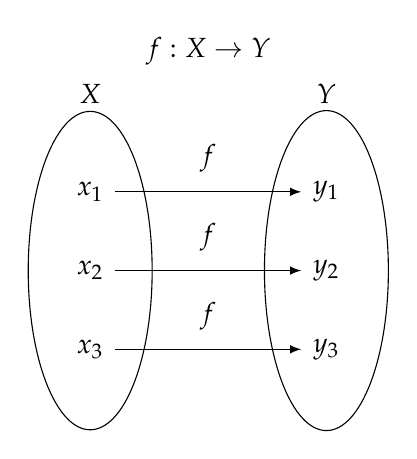
\begin{tikzpicture}[
            every node/.style={on grid},
            set/.style={circle,inner sep=2pt},
            every fit/.style={draw,ellipse,text width=25pt},
            >=latex
        ]
        
        % Draw domain %
        \node[set] (x1) {$x_1$};
        \node[set,below = of x1] (x2) {$x_2$};
        \node[set,below = of x2] (x3) {$x_3$};
        \node[above = of x1,anchor=south] (X) {$X$};

        % Draw co-domain %
        \node[set, right=3cm of x1] (y1) {$y_1$};
        \node[set, below = of y1] (y2) {$y_2$};
        \node[set, below = of y2] (y3) {$y_3$};
        \node[above = of y1,anchor=south] (Y) {$Y$};
        
        % Draw arrows %
        \draw[->] (x1) -- node[label=above:$f$] {} (y1);
        \draw[->] (x2) -- node[label=above:$f$] {} (y2);
        \draw[->] (x3) -- node[label=above:$f$] {} (y3);
        
        % Draw ellipses %
        \begin{pgfonlayer}{background}
            \node[fit = (x1) (x3) ] {};
            \node[fit = (y1) (y3) ] {};
        \end{pgfonlayer}

        % Label %
        \node[anchor=south] at (current bounding box.north) {$f:X \to Y$};
        \end{tikzpicture}
    \end{figure}

    \textbf{Examples: }
    \begin{itemize}
        \item $f: \N \to \N, f(n) = n!$ is a function
        \item $f: \R \to \R, f(x) = \ln{x}$ is not a function as $f(x)$ is 
        undefined for $x \lt 0$
        \item $f: \Q \to \N, f(\frac{n}{m}) = n$ is not a function as there are multiple
        ways to write the same input with different outputs, e.g. $\frac{3}{2} = 3$ but $\frac{6}{4} = 6$.
    \end{itemize}

    \subsubsection{Function Terminology}
    Let $f:X \to Y$ be a function. Then we say:
    \begin{itemize}
        \item $X$ is called the \textbf{domain} of $f$
        \item $Y$ is called the \textbf{co-domain} of $f$
        \item $f(x) \in Y$ is called the \textbf{image} of $X$ (also called range).\\
    \end{itemize}

    \begin{figure}[!hbt]
        \centering
        \begin{tikzpicture}[
            every node/.style={on grid},
            set/.style={circle,inner sep=2pt},
            every fit/.style={draw,ellipse,text width=25pt},
            >=latex
        ]
        
        % Draw domain %
        \node[set] (x1) {$x_1$};
        \node[set,below = of x2] (x3) {$x_3$};
        \node[above = of x1,anchor=south] (X) {$X$};

        % Draw co-domain and image of x %
        \node[set, right=3cm of x1] (cd1) {};
        \node[set, below= of cd1] (y1) {$f(x_1)$};
        \node[set, below= of y1] (y2) {$f(x_2)$};
        \node[set, below= of y2] (cd2) {};
        \node[above = of cd1,anchor=south] (Y) {$Y$};
        \node[above = of y1,anchor=south] (I) {Image};
        
        % Draw arrows %
        \draw[->] (x1) -- node[label=above:$f$] {} (y1);
        \draw[->] (x2) -- node[label=above:$f$] {} (y2);
        
        % Draw ellipses %
        \begin{pgfonlayer}{background}
            \node[fit = (x1) (x3) ] {};
            \node[fit = (cd1) (cd2), minimum width = 3cm, minimum height = 4cm] {};
            \node[fit = (y1) (y2)] {};
        \end{pgfonlayer}
        \end{tikzpicture}
    \end{figure}

    Similarly, the \textbf{pre-image} of a y is the set of all input values which
    map to the co-domain $Y$. This is written as 
    $f^{-1}(y)=\{x\in X \mid f(x) = y\} \subseteq X$. In essence, it explains where
    does $y$ come from under the function $f(x)$.

    \subsubsection{Identity Function}
    \begin{definition}[Identity Function]
        \label{def:identity-function}
        The \textbf{identity function} is a function which maps a set to iteself. For any set $S$,
        $i_x:X \to X$ is defined by $i_x(a) = a, a \in X$.       
    \end{definition}

    \subsubsection{Floors and Ceilings}
    \begin{definition}[Floor]
        \label{def:floor}
        For $x \in \R$, the floor of $x$ is the unique integer $n$ such that $n \le x \le n+1$.
        In essence, it is "rounding down" $x$ in terms of value. It is written as $\lfloor x \rfloor$. \\
    \end{definition}

    \begin{definition}[Ceiling]
        \label{def:ceiling}
        For $x \in \R$, the ceiling of $x$ is the unique integer $m$ such that $m-1 \le x \le m$.
        In essence, it is "rounding up" $x$ in terms of value. It is written as $\lceil x \rceil$.
    \end{definition}

    \textbf{Note: } both floor and ceiling are functions $f: \R \to \Z$. 
    Additionally, for $x \lt 0$, the rounding up/down of these functions are reversed.

    \textbf{Examples:}
    \begin{itemize}
        \item $\lfloor 2.5 \rfloor = 2$
        \item $\lfloor -2.5 \rfloor = -3$
        \item $\lceil 2.5 \rceil = 3$
        \item $\lceil -2.5 \rceil = -2$
    \end{itemize}

    \subsection{Properties of Functions}
    \subsubsection{Equality of Functions}
    \begin{definition}[Equal Functions]
        \label{def:equal-functions}
        Two functions, $f: X \to Y$ and $g: X \to Y$ are said to be equal if
        $f(x) = g(x)$ for all $x \in X$.
    \end{definition}

    \textbf{Example:} $f$ and $g$ are equal.
    \begin{itemize}
        \item $f(x) = n!$
        \item $g(x) = \frac{(n+1)!}{n+1} = \frac{(n+1)n!}{n+1}=n!$
    \end{itemize}

    \textbf{Example:} $f$ and $g$ are not equal (not same co-domain).
    \begin{itemize}
        \item $f:\N \to \N, f(n) = n^2$
        \item $g:\N \to \R, f(n) = n^2$
    \end{itemize}

    \subsubsection{Surjective/Onto}
    \begin{definition}
        \label{def:surjective}
        A function $f: X \to Y$ is considered \textbf{onto} or \textbf{surjective} if
        for all $y \in Y$, there exists some $f(x) = y$, $x \in X$. In other words,
        the co-domain has no orphans; every $y$ is the image of at least one $f(x)$.
    \end{definition}

    \textbf{Example:} \\
    The below function is \textbf{not} a surjective function since $y_3$ is "orphaned".
    \begin{figure}[!hbt]
        \centering
        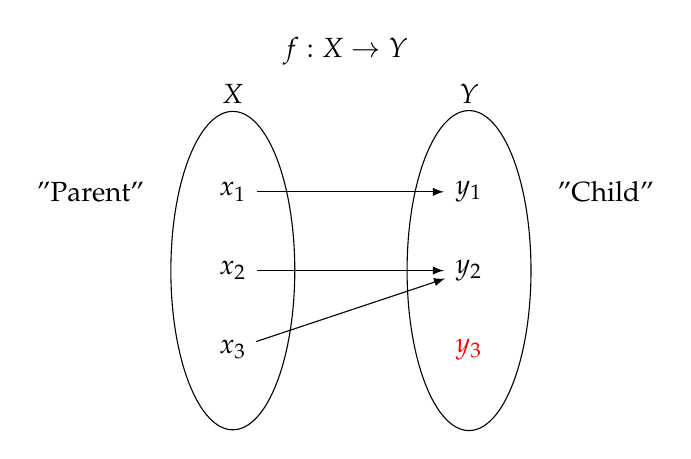
\begin{tikzpicture}[
            every node/.style={on grid},
            set/.style={circle,inner sep=2pt},
            every fit/.style={draw,ellipse,text width=25pt},
            >=latex
        ]
        
        % Draw domain %
        \node[set] (x1) {$x_1$};
        \node[set,below = of x1] (x2) {$x_2$};
        \node[set,below = of x2] (x3) {$x_3$};
        \node[above = of x1,anchor=south] (X) {$X$};
        \node[left = of x1,anchor=east] (X) {"Parent"};

        % Draw co-domain %
        \node[set, right=3cm of x1] (y1) {$y_1$};
        \node[set, below = of y1] (y2) {$y_2$};
        \node[set, below = of y2, color=red] (y3) {$y_3$};
        \node[above = of y1,anchor=south] (X) {$Y$};
        \node[right = of y1,anchor=west] (Y) {"Child"};
        
        % Draw arrows %
        \draw[->] (x1) -- node[] {} (y1);
        \draw[->] (x2) -- node[] {} (y2);
        \draw[->] (x3) -- node[] {} (y2);
        
        % Draw ellipses %
        \begin{pgfonlayer}{background}
            \node[fit = (x1) (x3) ] {};
            \node[fit = (y1) (y3) ] {};
        \end{pgfonlayer}

        % Label %
        \node[anchor=south] at (current bounding box.north) {$f:X \to Y$};
        \end{tikzpicture}
    \end{figure}

    \subsubsection{Injective/One-to-One}
    \begin{definition}
        \label{def:injective}
        A function $f: X \to Y$ is considered \textbf{one-to-one} or \textbf{injective} if
        $f(x_1) = f(x_2)$ implies $x_1 = x_2$ for all $x_1, x_2 \in X$. In other words,
        different elements in X must map to different images in Y (two elements can't map
        to same place).
    \end{definition}

    \textbf{Example:} The function below is \textbf{not} an injective function
    since $x_2$ and $x_3$ map to $y_2$, and $x_2 \ne x_3$.

        \begin{figure}[!hbt]
        \centering
        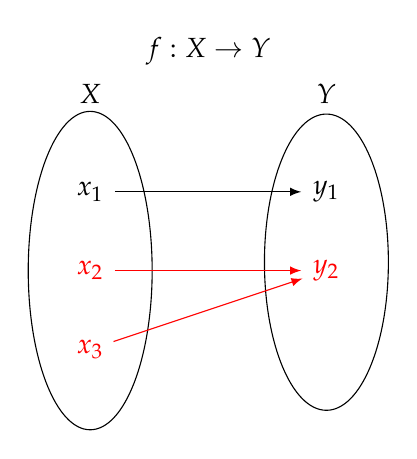
\begin{tikzpicture}[
            every node/.style={on grid},
            set/.style={circle,inner sep=2pt},
            every fit/.style={draw,ellipse,text width=25pt},
            >=latex
        ]
        
        % Draw domain %
        \node[set] (x1) {$x_1$};
        \node[set,below = of x1, color=red] (x2) {$x_2$};
        \node[set,below = of x2, color=red] (x3) {$x_3$};
        \node[above = of x1,anchor=south] (X) {$X$};

        % Draw co-domain %
        \node[set, right=3cm of x1] (y1) {$y_1$};
        \node[set, below = of y1, color=red] (y2) {$y_2$};
        \node[set, below = of y2] (y3) {};
        \node[above = of y1,anchor=south] (X) {$Y$};
        
        % Draw arrows %
        \draw[->] (x1) -- node[] {} (y1);
        \draw[->, color=red] (x2) -- node[] {} (y2);
        \draw[->, color=red] (x3) -- node[] {} (y2);
        
        % Draw ellipses %
        \begin{pgfonlayer}{background}
            \node[fit = (x1) (x3) ] {};
            \node[fit = (y1) (y3) ] {};
        \end{pgfonlayer}

        % Label %
        \node[anchor=south] at (current bounding box.north) {$f:X \to Y$};
        \end{tikzpicture}
    \end{figure}

    \subsubsection{Bijective}
    \begin{definition}
        \label{def:bijective}
        A function is said to have a \textbf{one-to-one correspondence} or \textbf{bijective}
        if it is both injective and surjective. In other words, if all elements $x\in X$ are paired
        with a unique $y \in Y$.
    \end{definition}

    \textbf{Example:} The below function is bijective.

    \begin{figure}[!hbt]
        \centering
        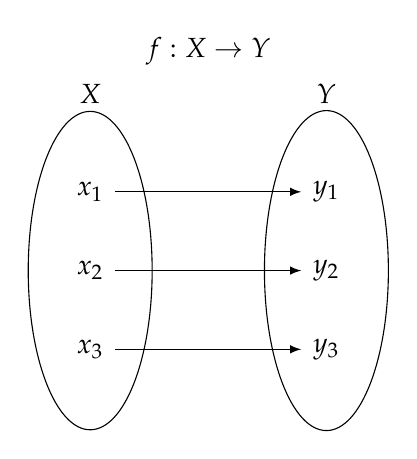
\begin{tikzpicture}[
            every node/.style={on grid},
            set/.style={circle,inner sep=2pt},
            every fit/.style={draw,ellipse,text width=25pt},
            >=latex
        ]
        
        % Draw domain %
        \node[set] (x1) {$x_1$};
        \node[set,below = of x1] (x2) {$x_2$};
        \node[set,below = of x2] (x3) {$x_3$};
        \node[above = of x1,anchor=south] (X) {$X$};

        % Draw co-domain %
        \node[set, right=3cm of x1] (y1) {$y_1$};
        \node[set, below = of y1] (y2) {$y_2$};
        \node[set, below = of y2] (y3) {$y_3$};
        \node[above = of y1,anchor=south] (X) {$Y$};
        
        % Draw arrows %
        \draw[->] (x1) -- node[] {} (y1);
        \draw[->] (x2) -- node[] {} (y2);
        \draw[->] (x3) -- node[] {} (y3);
        
        % Draw ellipses %
        \begin{pgfonlayer}{background}
            \node[fit = (x1) (x3) ] {};
            \node[fit = (y1) (y3) ] {};
        \end{pgfonlayer}

        % Label %
        \node[anchor=south] at (current bounding box.north) {$f:X \to Y$};
        \end{tikzpicture}
    \end{figure}

    \subsubsection{Proving Properties of Functions}
    \begin{center}
        \begin{tabular}{ | m{3cm} | m{6cm}| m{6cm} | }
            \hline
            \textbf{Property} & \textbf{Proving} & \textbf{Disproving}\\
            \hline
            \textbf{Surjective} & 
            Take any arbitrary $y \in Y$, construct some $x \in X$ so that $f(x)=y$ &
            Find a counterexample, $y \in Y$ and show $y \ne f(x)$ for any $x \in X$ \\
            \hline
            \textbf{Injective} &
            Assume $f(x_1) = f(x_2)$and deduce $x_1=x_2$ &
            Find a counterexample, $x_1, x_2 \in X$, where $x_1 \ne x_2$ but $f(x_1) = f(x_2)$ \\
            \hline
            \textbf{Bijective}&
            Prove both &
            Disprove at least one \\
            \hline
        \end{tabular}
    \end{center}

    \newpage
    \textbf{Example:} Let $f,g: \N \to \N$. Prove if $f$ and $g$ are 
    injective and surjective.
    
    \begin{center}
        \begin{tabular}{ | m{3cm} | m{12cm} |}
            \hline
            \multicolumn{2}{|c|}{$f(n)=n^2$} \\
            \hline
            \textbf{Surjective?} &
            No, the function is not surjective as the image of x only covers squares,
            whilst the codomain is $y \in \N$. For example, let $y$ be 3, then $f(n) = 3$,
             $n = \pm \sqrt{3}$, but $\pm \sqrt{3} \notin \N$. \\
            \hline
            \textbf{Injective?} &
            Yes the function is injective according to the proof.
            \begin{equation*}\begin{aligned}
                \text{Assume } f(n) = f(m) \\
                \implies n^2 &= m^2 \\
                n^2 - m^2 &= 0 \\
                (n+m)(n-m) &= 0 \\
                \implies n=-m \text{ or } m=-n \\
                \text{but $n \in \N$, so $n \ne -m$}
            \end{aligned}\end{equation*}
            Since $n$ can only equal $m$, we know that the function is injective. \\
            \hline
        \end{tabular}
    \end{center}
    
    \begin{center}
        \begin{tabular}{ | m{3cm} | m{12cm} |}
            \hline
            \multicolumn{2}{|c|}{$g(n)=\abs{n-1}$} \\
            \hline
            \textbf{Surjective?} &
            Yes, the function is surjective according to the proof.
            \begin{equation*}\begin{aligned}
                \text{Let } y & \in \N \\
                \text{If } y \in \N, \text{ then } y+1 & \in \N \\
                g(y+1) & = \abs{(y+1)-1} \\
                & = \abs{y} \\
                & = y
            \end{aligned}\end{equation*} \\
            \hline
            \textbf{Injective?} &
            No, the function is not injective, consider $g(n) = 1$, then $g(0)$ and $g(2)$
            both satisfy $f(n)=1$, but $0 \ne 2$.\\
            \hline
        \end{tabular}
    \end{center}
    
    \subsubsection{Functions and Finite Sets}
    Let $X, Y$ be two finite sets, and $f: X \to Y$.
    \begin{itemize}
        \item If $f$ is \textbf{injective}, then $\abs{X} \le \abs{Y}$
        \item If $f$ is \textbf{surjective}, then $\abs{X} \ge \abs{Y}$
        \item If $f$ is \textbf{bijective}, then $\abs{X} = \abs{Y}$
    \end{itemize}

    \subsubsection{Compositions of Functions}
    \begin{definition}[Composite Function]
        \label{def:composite-function}
        Let $f:X \to Y$ $g: Y \to Z$ be two functions. The composition is written
        $g \circ f: X \to Z$
    \end{definition}
    \textbf{Example:} Let $f:\R^2 \to \R, f(x,y) = xy$ 
    and $g:\R \to \R^2, g(x) = (\sin{x}, x)$ be functions.

    \begin{equation*}
        \begin{aligned}
            f \circ g &: \R^2 \to R^2 \\
            f(g(x)) &= f((\sin{x}, x))\\
            &= \sin{x} \times x \\\\
            g \circ f &: \R \to \R \\
            g(f(x)) &= g(xy)\\
            &= (\sin{xy}, xy)
        \end{aligned}
    \end{equation*}

    \subsection{Sequences}
    \subsubsection{Sequences}
    \begin{definition}[Sequence]
        \label{def:sequence}
        A \textbf{sequence} is an ordered list of data. That is, given a set $S$,
        a sequence in $S$ is a function $f: I \to S$ where $I \subseteq \Z$ (we can assign
        a numerical order for elements in the set S).
    \end{definition}

    \textbf{Notation:} we use letters and subscripts to indicate elements of a sequence,
    for example $a_1 = f(1), a_2 = f(2), a_n = f(n)$. The terms of a sequence are its elements.

    \subsubsection{Equality of Sequences}
    To prove that two sequences, $p_n$ and $b_n$ are equal sequences, we need
    $b_n$ in closed form, and $p_n$ as a recursive sequence. Then we need to show that
    $b_n$ satisfies the recursion relation and initial condition.

    \textbf{Example:}
    \begin{itemize}
        \item Let $(p_n)=(2p_{n-1}+1)$, where $p_1 = 1$
        \item Let $(b_n)_{n \ge 1}=(2^n-1)$
    \end{itemize}
  
    \textbf{Prove} $p_n = b_n$ \\
    \textbf{Initial condition:} $b_1=(2^1-1)=1=p_1=1$ \\
    \textbf{Recursive relation:} Sub $b_{n-1}$ into $p_n$ if it equals $b_n$
    then it is a recursive relation. 
    \begin{equation*}
        \begin{aligned}
            2(b_{n-1}) +1 &= 2(2^{n-1}-1)+1 \\
            &=2^{n-1+1}-2+1 \\
            &=2^n-1 \\
            &=b_n
        \end{aligned}
    \end{equation*}

    \subsubsection{Summatiom}
    \begin{definition}
        \label{def:summation}
        The summation of a sequence $a_n$ is given by $\sum^{N}_{i=1}a_n$. In discrete math, we are 
        interested in finite summations and the closed formulas for them
    \end{definition}

    \textbf{Example:} Find a closed formula for $\sum_{i=1}^{N}i=1+2+\dots+N$.\\
    \textbf{Claim: $\sum_{i=1}^{N}i = \frac{N(N+1)}{2}$}
    \begin{proof}
        Let $M = \sum_{i=1}^{N}i$. \\
        Then,
        \begin{align*}
            2M &= 2 \times \sum_{i=1}^{N}i \\
            &= \sum_{i=1}^{N}i + \sum_{k=1}^{N}k \\\\
            \sum_{k=1}^{N}k &= N + (N-1) + (N-2) + \dots + 1 \\
            &= \sum_{k=1}^{N} (N - k + 1) \\\\
            2M &= \sum_{i=1}^{N} i + \sum_{k=1}^{N} (N - k + 1) \\
            &= \sum_{i=1}^{N} N + 1 = N(N+1) \\
            M &= \frac{N(N+1)}{2}
        \end{align*}
        \textbf{Note$_{1}$:} we changed variable $i$ to $k$ in the second summation. \\
        \textbf{Note$_{2}$:} the variables $i$ and $k$ are equal to each other, so when we add
        them in the final $2M$ calculation they cancel each other out.
    \end{proof}

    \newpage
    \section{Week 3}
    \subsection{Divisibility and Modular Arithmetic}
    \subsubsection{Divides}
    \textbf{Remark:} When discussing division, we only use integers $\Z$.\\
    \begin{definition}[Divides]
        \label{def:divides}
        For two integers $a$ and $b$, we say that $a$ \textbf{divides} $b$,
        written as $a \mid b$, if there exists some integer $k \in \Z$ such that
        $b = ak$. Otherwise, if $a$ does not divide $b$ we write $a \nmid b$.
    \end{definition}

    \textbf{Examples:}
    \begin{itemize}
        \item $-3 \mid 12$ since $-4(-3) = 12$
        \item $4 \nmid 7$ since there is not integer such that $7 = 4k$
        \item $1 \mid n$ for all $n \in \Z$ since $n = 1(k)$
        \item $n \mid 0$ for all $n$ since $0 = n(0)$
    \end{itemize}

    \subsubsection{Properties of Divisibility}
    Let $a,b,c \in \Z$, and $a \ne 0$:
    \begin{enumerate}
        \item If $a \mid b$ and $a \mid c$, $\implies a \mid (b+c)$
        \item If $a \mid b$, $\implies a \mid bc$
        \item If $a \mid b$, $b \ne 0$ and $b \mid c$, $\implies a \mid c$
    \end{enumerate}
    \begin{proof}[Proof. Property 1]
        Assume $a \mid b$, and $a \mid c$. \\
        Then there exists some integers $k,j \in \Z$ such that:
        \begin{align*}
            b &= ak \\
            c &= aj
        \end{align*}
        Then, $b+c$ can be expressed as:
        \begin{align*}
            b + c &= ak + aj \\
            &= a(k+j)
        \end{align*}
        Which fits our definition of divisibility, thus $a \mid (b+c)$.
    \end{proof}

    \begin{proof}[Proof. Property 2]
        Assume $a \mid b$. \\
        Then it follows that $a \mid bc$ since $bc = (ak)c = a(kc)$. Which fits our definition
        of divisibility.
    \end{proof}

    \begin{proof}[Proof. Property 3]
        Assume that $a \mid b$, $b \ne 0$ and $b \mid c$. \\
        Then, we say:
        \begin{align*}
            b &= ak \text{ for some } \{k \in \Z \mid k \ne 0\} \\
            c &= bj \text{ for some } \{j \in \Z\} \\
            &= (ak)j
        \end{align*}
        This fits our definition of divisibility, thus $a \mid c$.
    \end{proof}

    \subsubsection{The Remainder Theorem}
    The remainder theorem is applied when $a \nmid b$. \\
    \begin{theorem}[Remainder Theorem]
        \label{thm:remainder-theorem}
        Let $n,d,\in \Z$ be two integers with $d > 0$. Then there are unique integers $q, r$ with
        $0 \le r \lt d$. Such that $n = dq + r$.
    \end{theorem}

    \textbf{Note:} Remainders must be:
    \begin{itemize}
        \item Non-negative $0 \le r$
        \item Less than the divisor $r \lt d$
    \end{itemize}

    \textbf{Example 1:} $12 \nmid 51$
    \begin{align*}
        51 = 12(4) + 3 \\
        d = 12, q = 4, r = 3
    \end{align*}

    \textbf{Example 2:} \\
    An application of this is determing if there is an integer $n$ such that 
    $\{n^2 \in Z \mid \text{ends with 7}\}$ Some examples are shown below:
    \begin{align*}
        &&0^2 &&1^2 &&2^2 &&3^2 &&4^2 &&5^2 &&6^2 &&7^2 &&8^2 &&9^2 &&10^2 \\
        &&0 &&1 &&4 &&9 &&16 &&25 &&36 &&49 &&64 &&81 &&100
    \end{align*}
    We notice that the pattern starts repeating after 9 digits, none end in 7. \\
    Let $n \in \Z$, then $n = 10q + r$, where $r$ is the last digit of $n \implies 
    0 \le r \lt 10$.
    \begin{align*}
        n^2 &= (10q + r)(10q + r) \\
        &= (100q^2 + 20qr + r^2) \\
        &= 10(10q^2 + 2qr) + r^2
    \end{align*}
    The last digit of $n^2$ is determined by $r^2$. From the examples above, we know
    $r$ will not equal 7, thus there is no integer $n$ such that $n^2$ ends with 7.

    \subsubsection{Modular Arithmetic}
    \begin{definition}[Congruence Modulo]
        \label{def:congruence-modulo}
        If two integers $n , m \in \Z$ have the same remainder when divided by $d$, we say
        $n$ and $m$ are \textbf{congruent modulo d} and write $m \equiv n \mod d$. In other words,
        \begin{align*}
            n &= q_1(d) + r \\
            m &= q_2(d) + r \\
            &\implies n \equiv m \mod d
        \end{align*}
    \end{definition}

    \textbf{Properties of Congruence Modulo:}
    \begin{enumerate}
        \item $n = qd +r \implies n \equiv r \mod d$
        \item $n \equiv m \mod d \iff d \mid (n - m)$
        \item $n \equiv 0 \mod \iff d \mid n$
    \end{enumerate}

    \subsection{Prime Numbers, GCD, LCM}
    \subsubsection{Prime Numbers}
    \begin{definition}[Prime Number]
        \label{def:prime-number}
        A number $p \in \N$  is \textbf{prime} if $p \gt 1$ and the only divisors of $p$
        are $\pm 1$ and $\pm p$. Otherwise, $p$ is called \textbf{composite}.
    \end{definition}
    \textbf{Examples:}
    \begin{itemize}
        \item 2, 3, 5, 7, 11, 13, 17, 19, 23, 29 are prime numbers
        \item 4, 6, 8, 9, 10, 12, 14, 15, 16, 18 are composite numbers
    \end{itemize}

    \subsubsection{Fundamental Theorem of Arithmetic}
    \begin{theorem}[Fundamental Theorem of Arithmetic]
        \label{thm:fundamental-theorem-of-arithmetic}
        Every integer $n \gt 1$ can be uniquely written as a product of primes.
        \begin{equation*}
            n = p_1^{k_1} p_2^{k_2} \dots p_m^{k_m} = \prod_{i=1}^{m} p_i^{k_i}
        \end{equation*}
    \end{theorem}

    \subsubsection{Positive Divisors of $n$}
    If we know the prime decomposition of $n$ we can determine the number of positive 
    divisors of $n$.

    For example $72 = 2^3 \times  3^2$. There are:
    \begin{itemize}
        \item 4 choices for the power of 2: $2^0, 2^1, 2^2, 2^3$
        \item 3 choices for the power of 3: $3^0, 3^1, 3^2$
    \end{itemize}
    Thus, in total there are $4(2) + 3(3) = 12$ possible positive divisors of 72.

    \subsubsection{GCD}
    \begin{definition}[Greatest Common Divisor]
        \label{def:greatest-common-divisor}
        The \textbf{greatest common divisor} of two integers $a,b \in \Z$, not both zero,
        is the largest integer $d$ such that $d \mid a$ and $d \mid b$. It is written as
        $\gcd(a,b)$ or $(a,b)$.
    \end{definition}

    \subsubsection{LCM}
    \begin{definition}[Least Common Multiple]
        \label{def:least-common-multiple}
        is the smallest positive integer $m$ such that $a \mid m$ and $b \mid m$. It is written as
        $\lcm(a,b)$.
    \end{definition}

    \subsubsection{Computing GCD and LCM using Prime Factorisation}
    Let $a, b \in \Z$. Then the GCD and LCM can be computing using their prime factorisations:
    \begin{itemize}
        \item \textbf{For GCD:} take the minimum power of all primes \textbf{in common between}
        $a$ and $b$, ignore negative signs.
        \item \textbf{For LCM:} take the maximum power of all primes in $a$ and $b$.
    \end{itemize}

    \textbf{Example:} Two integers are given:
    \begin{itemize} 
        \item $576 = 2^6 \times 3^2$
        \item $78408 = 2^3 \times 3^4 \times 11^2$
    \end{itemize}
    Their GCF and LCM are given:
    \begin{itemize}
        \item $\gcd(576,78408) = 2^3 \times 3^2$
        \item $\lcm(576, 78408) = 2^6 \times 3^4 \times 11^2$
    \end{itemize}

    \subsection{Euclidean Algorithm}
    \subsubsection{Euclidean Algorithm}
    \begin{definition}[co-prime]
        \label{def:co-prime}
        Two integers $a,b \in \Z$ are said to be \textbf{co-prime} if $\gcd(a,b) = 1$,
        e.g. $\gcd(5,7) = 1$\\
    \end{definition}

    \begin{theorem}
        \label{thm:euclidean-algorithm}
        $\gcd(a,b) = \gcd(b, r)$. \\
    \end{theorem}
    \begin{proof}
        Suppose there exists some $d \in \Z$ such that $d \mid a$ and $d \mid b$,
        \begin{align*}
            d &\mid (a + qb), \{q \in \Z\} \\
            d &\mid r \text{ since $r = a - qb$}
        \end{align*}
        \textbf{Note:} $(a+qb)$ follows the property 1 of divisibility $d \mid (a + b)$\\
        Now consider the existence of some $c \in \Z$ such that $c \mid b$ and $c \mid r$.
        \begin{align*}
            c &\mid (r + qb) \\
            c &\mid ((a - qb) + qb) \text{ since $r = a-qb$}\\
            c &\mid a
        \end{align*}
        Now both $d$ and $c$ share common divisors, thus $\gcd(a,b) = \gcd(b,r)$.
    \end{proof}

    \subsubsection{Application of Euclidean Algorithm}
    \textbf{To Find $\gcd(a,b)$ with $a \ge b \ge 0$:}
    \begin{enumerate}
        \item Write $a = qb + r$ by division algorithm
        \item If $r = 0$, then $\gcd(a,b) = b$. Stop.
        \item Otherwise if $r \ne 0$, then replace $a$ by $b$ and repeat.
    \end{enumerate}

    \textbf{Example:} See assignment 1 Q3.

    \subsubsection{Base b Expansions}
    \begin{definition}[Base b Expansion]
        \label{def:base-b-expansion}
        Numbers are typically denoted "decimally", i.e. in "base1-10".
        \begin{equation*}
            n = a_0 \times 10^0 + a_1 \times 10^1 + a_2 \times 10^2 + \dots + a_k \times 10^k
        \end{equation*}
        Let $b > 1$ be a positive integer. Then every positive integer $n$ can be
        uniquely expressed as:
        \begin{equation*}
            n = a_0 \times b^0 + a_1 \times b^1 + a_2 \times b^2 + \dots + a_k \times b^k
        \end{equation*} 
    \end{definition}

    \textbf{Example 1:} Convert $78_{10}$ to base 2.
    \begin{align*}
        78 &= 2(39) + 0 \\
        39 &= 2(19) + 1 \\
        19 &= 2(9) + 1 \\
        9 &= 2(4) + 1 \\
        4 &= 2(2) + 0 \\
        2 &= 2(1) + 0 \\
        1 &= 2(0) + 1 \\
        &\implies 78_{10} = 1001110_2
    \end{align*}
    Here, we take the remainder from bottom to top to get the base 2 representation.

    \textbf{Example 2:} Convert $(245)_8$ to base 10.
    \begin{align*}
        245_8 &= (5 \times 8^0) + (4 \times 8^1) + (5 \times 8^2) \\
        &= 5 + 32 + 128 \\
        &= 165_{10}
    \end{align*}

    \subsubsection{Base b Arithmetic}
    Base $b$ expressions are positional. The usual arithmetic operations work, but you
    need to "carry over" $b$ instead of 10.

    \newpage
    \section{Week 4}

    \newpage
    \section{Week 5}
    
\end{document}